\chapter{Evaluation and calibration of a new routing scheme over the Iberian Peninsula}
\label{chap:routing}
\minitoc
\pagebreak

\section{Chapter introduction}

This chapter presents the preliminary work to evaluate and calibrate the new version of the routing scheme (\native) before running coupled simulations with ICOLMDZOR. As a reminder, the pre-existing version of the routing scheme \std cannot be used with ICOLMDZOR because it imposes constraints on the ORCHIDEE and routing grids that are incompatible with the icosahedral grid.
The \native routing is based on the same modelling principles (described in Chapter \ref{chap:methods}) as \std but relies on a new code to interpolate between the ORCHIDEE grid and the routing grid. 

This preliminary work had two main objectives:
\begin{itemize}
    \item Ensure that the new code could replicate the behaviour of the \std version if given the same parameters and DEM as input. 
    Indeed, this routing has long been the default version in ORCHIDEE and in the IPSL-CM, including for CMIP6 coupled model runs and has been subject to calibration and evaluation studies. %todo:ref ?
    \item Evaluate and calibrate the new code using a high resolution DEM over the Iberian Peninsula to identify an appropriate set of parameters for coupled simulations.
\end{itemize}

%tood:reprendre pour mieux poser une question scientifique

\section{Methods for the routing scheme evaluation and calibration}

%todo: explain 2 DEMs better

The relevant routing outputs for evaluation and calibration are river discharge and water volumes in each of the reservoirs (groundwater, surface runoff, rivers). 
It must be noted that these volumes cannot be easily compared to observations, since large-scale measurements of groundwater or river volumes are complex and may not physically correspond to the abstraction level of the reservoirs modelled in ORCHIDEE.
There importance in this work is mainly justified by the fact that the irrigatin scheme withdraws water from these reservoirs to satisfy the irrigation demand while conserving water quantities.

All simulations for this chapter are run in offline mode, meaning that ORCHIDEE is not coupled to any atmospheric model but takes meteorological data as input. The choice of this meteorological forcing may impact the results of the offline simulation.

In all this chapter, the simulated river discharge is evaluated against monthly observation data from discharge stations of the Global Runoff Data Center \cite[GRDC, https://grdc.bafg.de,][]{fekete_global_2003}.
Stations were positioned on the 0.5° DEM grid using only the GPS position, and on the MERIT DEM grid with tools presented in \cite{polcher_hydrological_2023}, which use the GPS position of the stations as well as the upstream catchment area to find the most appropriate grid cell for comparison with the observations. 
Four stations were used between 2003 and 2012, which are all on large rivers (Ebro, Douro, Tagus, Guadiana) and show large discharge values, meaning they represent the integrated discharge over a large share of the basins. 

\begin{figure}[htbp]
    \centering
    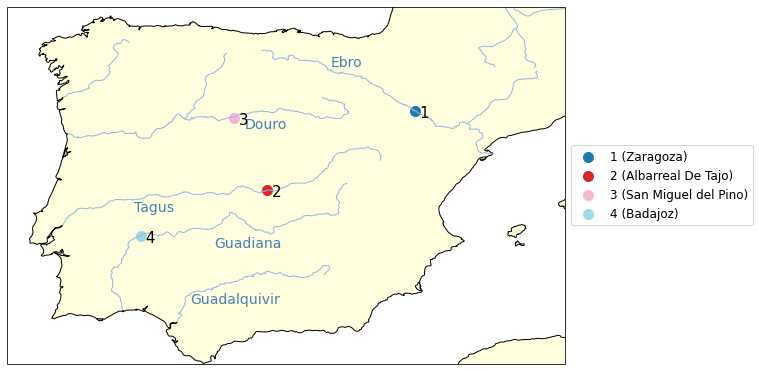
\includegraphics[width=0.7\linewidth]{images/eval_halfdeg/river_discharge/halfdeg_4stations_map.png}
    \caption{Discharge stations selected for the routing scheme evaluation and calibration.}
    \label{fig:halfedg_stations_map}
\end{figure}

%todo : expliquer période 2000-2012 + spinup -> forçages historiques et obs beaucoup plus dispo (et on n'était pas encore sûrs de la période pour les simus couplées...)

\section{Consistency of \native with \std routing}
\subsubsection{Simulation setup}

This first analysis used the \native routing in the same setup as the \std routing. 
The input DEM was the same (0.5° resolution), and the time constants for the three reservoirs were the same as the default values for the global model (Table \ref{table:tcst_refs}). Four simulations were run, two without irrigation (labeled as \textit{no\_irr}) to assess the routing schemes without its influence, and two with irrigation (labeled as \textit{irr}). It must be noted that these simulations were not aimed at evaluating the realism of simulated irrigation (which will be addressed in Section \ref{section:calib}) but only to assess if the new routing code behaves similarly to the previous version.

\begin{table}[h]
\centering
\begin{tabular}{|c|c|c|}
\hline
\textbf{TCST\_SLOW} & \textbf{TCST\_FAST} & \textbf{TCST\_STREAM} \\ \hline
25            & 3             & 0.24            \\ \hline
\end{tabular}
\caption{Routing time constant for the consistency analysis ($day \cdot km^{-1}$).}
\label{table:tcst_consistency}
\end{table}

Simulations were run from 2000 to 2012, with the WFDEI forcing. %todo:version/ref
The first three years were considered as a spinup and removed from the analysis, to allow the vegetation and hydrological variables to reach an equilibrium. The regional domain covers the Iberian Peninsula and part of Morocco, since at the time, this region was also considered as a study area for coupled simulations. Since this idea was not pursued, the analysis only focuses on the Iberian Peninsula.

\subsubsection{Results}

%figure : 12 maps of mean reservoir volumes and hydrographs, for both sims and diff
%todo:subcaptions
\begin{figure}[htbp]
    \centering
    \begin{tabular}{ccc}
        \begin{subfigure}[b]{0.33\textwidth}
            \caption{}
            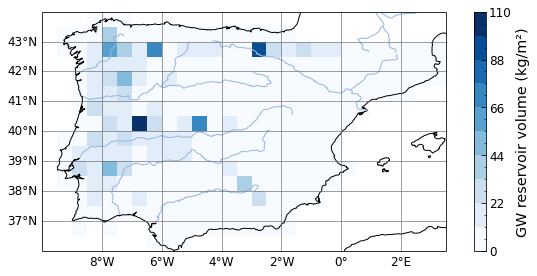
\includegraphics[width=\linewidth]{images/eval_halfdeg/maps/slowr_subgrid.png}
        \end{subfigure} &
        \begin{subfigure}[b]{0.33\textwidth}
            \caption{}
            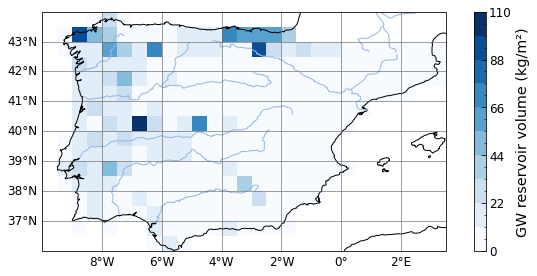
\includegraphics[width=\linewidth]{images/eval_halfdeg/maps/slowr_interp.png}
        \end{subfigure} &
        \begin{subfigure}[b]{0.33\textwidth}
            \caption{}
            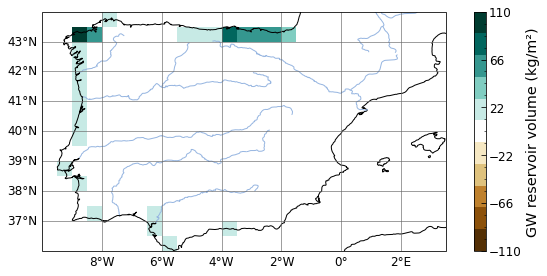
\includegraphics[width=\linewidth]{images/eval_halfdeg/maps/slowr_diff.png}
        \end{subfigure} \\
        
        \begin{subfigure}[b]{0.33\textwidth}
            \caption{}
            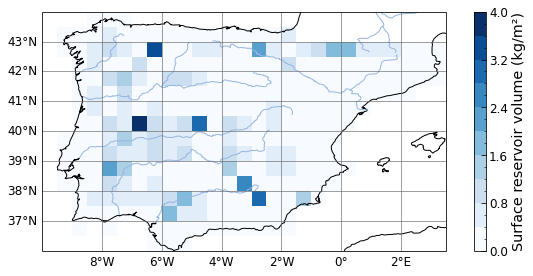
\includegraphics[width=\linewidth]{images/eval_halfdeg/maps/fastr_subgrid.png}
        \end{subfigure} &
        \begin{subfigure}[b]{0.33\textwidth}
            \caption{}
            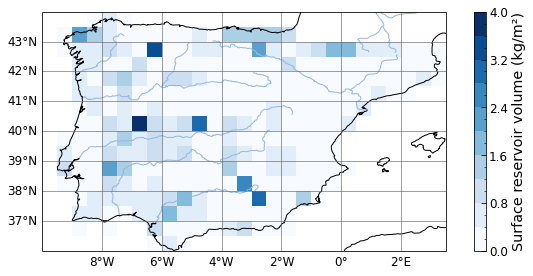
\includegraphics[width=\linewidth]{images/eval_halfdeg/maps/fastr_interp.png}
        \end{subfigure} &
        \begin{subfigure}[b]{0.33\textwidth}
            \caption{}
            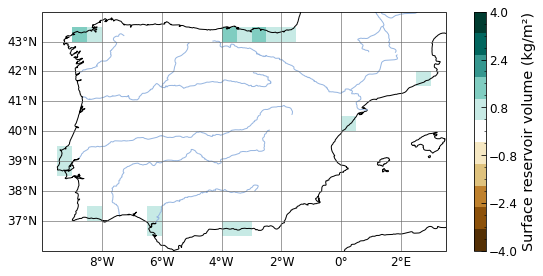
\includegraphics[width=\linewidth]{images/eval_halfdeg/maps/fastr_diff.png}
        \end{subfigure} \\
        
        \begin{subfigure}[b]{0.33\textwidth}
            \caption{}
            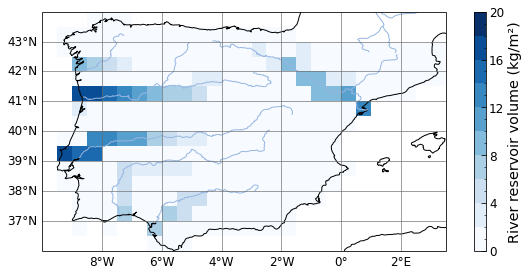
\includegraphics[width=\linewidth]{images/eval_halfdeg/maps/streamr_subgrid.png}
        \end{subfigure} &
        \begin{subfigure}[b]{0.33\textwidth}
            \caption{}
            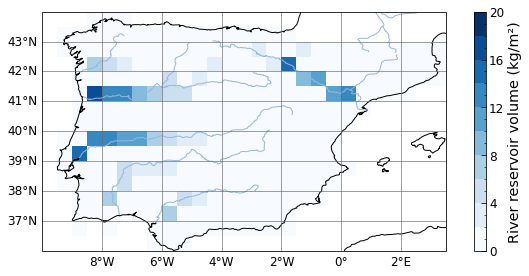
\includegraphics[width=\linewidth]{images/eval_halfdeg/maps/streamr_interp.png}
        \end{subfigure} &
        \begin{subfigure}[b]{0.33\textwidth}
            \caption{}
            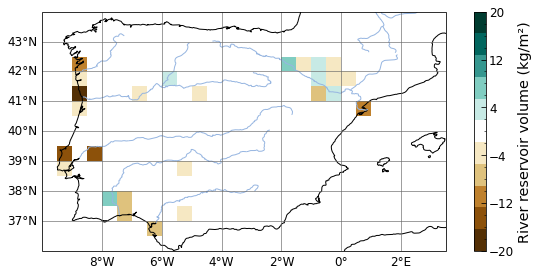
\includegraphics[width=\linewidth]{images/eval_halfdeg/maps/streamr_diff.png}
        \end{subfigure} \\
        
        \begin{subfigure}[b]{0.33\textwidth}
            \caption{}
            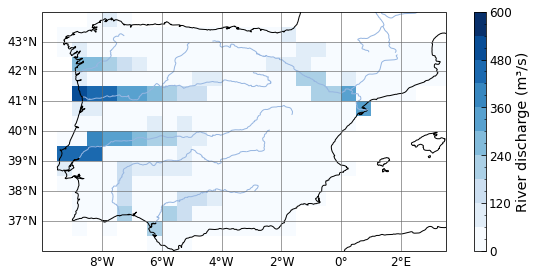
\includegraphics[width=\linewidth]{images/eval_halfdeg/maps/hydrographs_subgrid.png}
        \end{subfigure} &
        \begin{subfigure}[b]{0.33\textwidth}
            \caption{}
            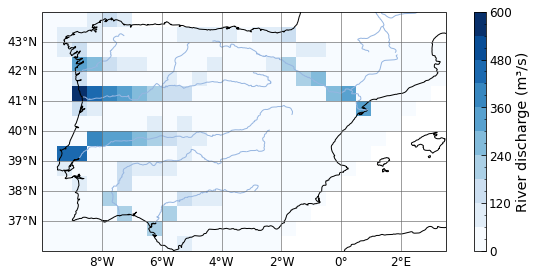
\includegraphics[width=\linewidth]{images/eval_halfdeg/maps/hydrographs_interp.png}
        \end{subfigure} &
        \begin{subfigure}[b]{0.33\textwidth}
            \caption{}
            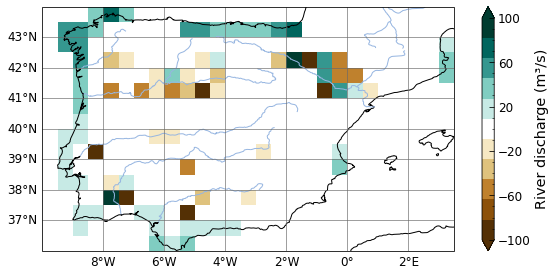
\includegraphics[width=\linewidth]{images/eval_halfdeg/maps/hydrographs_diff.png}
        \end{subfigure} \\
    \end{tabular}
    \caption{Annual mean (2003-2012) of reservoir volumes and river discharge for \std (\noirr), \native (\noirr) and difference between them.}
    \label{fig:routing_reservoirs_halfdeg}
\end{figure}

The comparison of the mean volumes for the fast and slow reservoirs (Fig. \ref{fig:routing_reservoirs_halfdeg}a-f) shows differences only on coastal grid cells, which have null values in \std but can have significant values in \native, particularly in the northern moutain ranges, which are regions of high precipitation, and therefore high drainage and surface runoff. %null, almost, ???
This is explained by a new modelling choice in the \native code, to represent these two reservoirs on coastal grid cells whereas drainage and surface runoff were considered to flow directly in the ocean in \std. %todo:check if this is true for standard... if not, we're missing an explanation...

Regarding the stream reservoir (Fig. \ref{fig:routing_reservoirs_halfdeg}g-i), an opposite choice was made on coastal grid cells. In \std, there was a stream reservoir for these grid cells, whereas it was removed in \native. This choice was made during the development of the scheme and might be changed in future versions to ensure consistency with the other two reservoirs. 
This change in coastal grid cells does not have an impact on the river discharge (Fig. \ref{fig:routing_reservoirs_halfdeg}j-l) because the way to compute it (\textit{hydrographs} variable in the model) was also changed from grid cell output to grid cell input. Coastal grid cell therefore have similar values of river discharge, but not of volume in the river reservoir. 
%todo:commenter l'augmentation de hydrographs sur les côtes. 

The most noticeable discrepancy on the stream reservoir and river discharge is that some non-coastal points have different values in both versions. It can be seen on Fig. \ref{fig:routing_reservoirs_halfdeg}j-l particularly that the water does not flow exactly in the same path, meaning that the DEM is not interpreted exactly in the same way by both versions. This has been attributed to small preprocessings of the DEM implemented in \std to avoid creating dead-ends, grid cells where the water would not keep flowing and accumulate in the stream reservoir. This was implemented when developing the routing scheme for global applications, possibly with a focus on other ORCHIDEE grid resolutions (1° or 2° instead of the 0.5° used here) and do not seem necessary for this domain and resolution, which is why they were not implemented in \native. These modifications may impact the routing graph, even though there do not seem to be any dead-ends in the routing graph computed by \native. In the large rivers where there are differences, \native seems to use shorter paths that \std, flowing diagonally to the next grid cell instead of taking two 90° turns. In most places, on annual average, this seems to lead to smaller amounts of water in the river reservoir and smaller discharge in \native compared to \std, as clearly visible on the Duero river in Fig. \ref{fig:routing_reservoirs_halfdeg}l.

%figure : 3 time series (3 reservoirs)on average over the IP for both routings
%todo:subcaptions
\begin{figure}[htbp]
    \centering
    \begin{subfigure}[b]{0.32\textwidth}
        \caption{}
        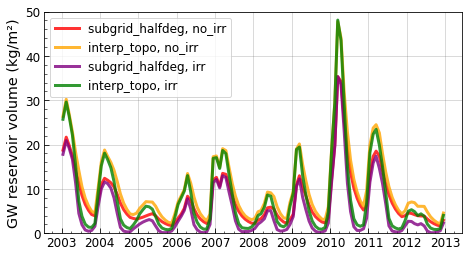
\includegraphics[width=\linewidth]{images/eval_halfdeg/time_series/slowr_time_series.png}
    \end{subfigure}
    \begin{subfigure}[b]{0.32\textwidth}
        \caption{}
        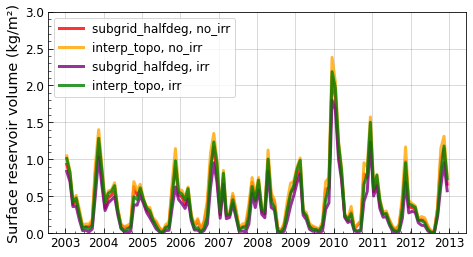
\includegraphics[width=\linewidth]{images/eval_halfdeg/time_series/fastr_time_series.png}
    \end{subfigure}
    \begin{subfigure}[b]{0.32\textwidth}
        \caption{}
        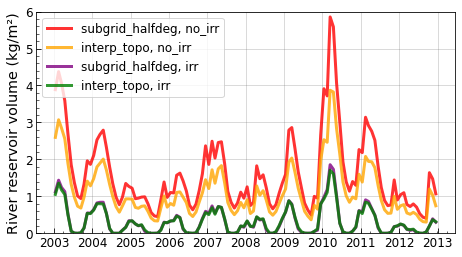
\includegraphics[width=\linewidth]{images/eval_halfdeg/time_series/streamr_time_series.png}
    \end{subfigure} \\

    \begin{subfigure}[b]{0.32\textwidth}
        \caption{}
        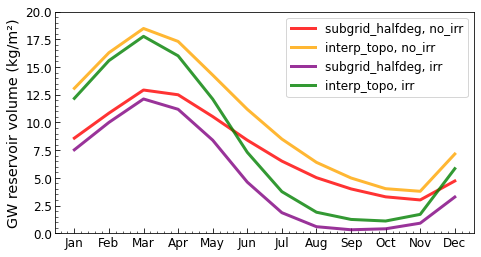
\includegraphics[width=\linewidth]{images/eval_halfdeg/time_series/slowr_seasonal_cycle.png}
    \end{subfigure}
    \begin{subfigure}[b]{0.32\textwidth}
        \caption{}
        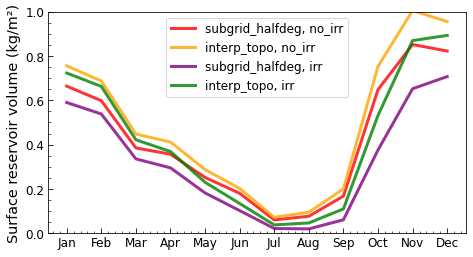
\includegraphics[width=\linewidth]{images/eval_halfdeg/time_series/fastr_seasonal_cycle.png}
    \end{subfigure}
    \begin{subfigure}[b]{0.32\textwidth}
        \caption{}
        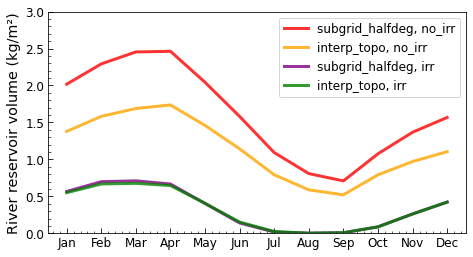
\includegraphics[width=\linewidth]{images/eval_halfdeg/time_series/streamr_seasonal_cycle.png}
    \end{subfigure}
    \caption{Time series and seasonal cycles of reservoir volumes on average over the Iberian Peninsula domain.}
    \label{fig:reservoir_time_series}
\end{figure}

On average over the Peninsula, these differences are visible in the groundwater and surface reservoirs where \native has larger volumes due to water in coastal grid cells (Fig. \ref{fig:reservoir_time_series}a, b). On the river reservoir however, \std has larger volumes, mostly due to the absence of this reservoir on coastal points with river outlets, which are the grid cells with the largest volumes in \std.
If all coastal grid cells were to be removed from the average (not shown)%todo: faire la figure ? ou annexe ?
, there would be no difference on the groundwater and surface reservoirs, and a much difference on the river reservoir, although \std still has more water stored in this reservoir than \native, particularly in winter and spring, when there is more rain in the region. This confirms the previous observation that water follows shorter paths to the sea in \native and therefore, does not remain in the river reservoir as long as in \std.
In the \irr simulations (purple and green lines in Fig. \ref{fig:reservoir_time_series}), all reservoirs are partly depleted by the irrigation withdrawals. For the groundwater and surface reservoirs, the differences between \std and \native mostly remain, since they are located in coastal grid cells, which are seldom intensely irrigated.
Regarding the river reservoir (Fig. \ref{fig:reservoir_time_series}f), \std simulates much lower volumes in the \irr than in \noirr simulation (-75\% in winter and complete depletion in summer). This decrease is also seen with \native, and the differences between the two routing versions almost disappear. This is consistent with the source of these differences, since the \irr simulations simulate much lower volumes in rivers, the discrepancies in the routing graph and at the river outlets have much less impact on the average volume over the domain.

%figure : 3 maps of simulated irrigation (subgrid, interp, diff), TS and SC of irrig for both simulations
%todo:subcaptions
\begin{figure}[htbp]
    \centering
    \begin{subfigure}[b]{0.32\textwidth}
        \caption{}
        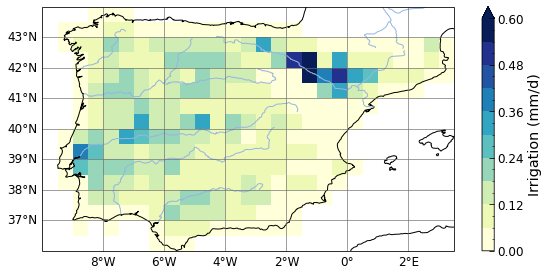
\includegraphics[width=\linewidth]{images/eval_halfdeg/maps/irrigation_subgrid.png}
    \end{subfigure}
    \begin{subfigure}[b]{0.32\textwidth}
        \caption{}
        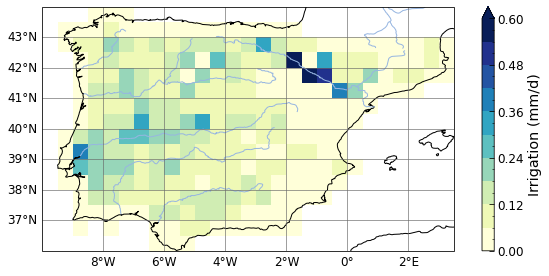
\includegraphics[width=\linewidth]{images/eval_halfdeg/maps/irrigation_interp.png}
    \end{subfigure}
    \begin{subfigure}[b]{0.32\textwidth}
        \caption{}
        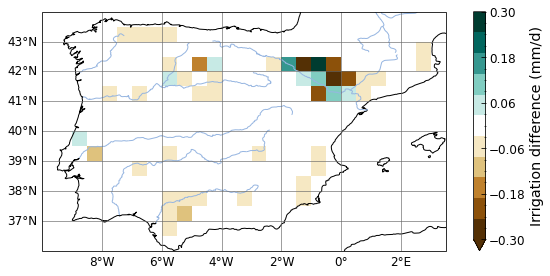
\includegraphics[width=\linewidth]{images/eval_halfdeg/maps/irrigation_diff.png}
    \end{subfigure} \\

    \begin{subfigure}[b]{0.48\textwidth}
        \caption{}
        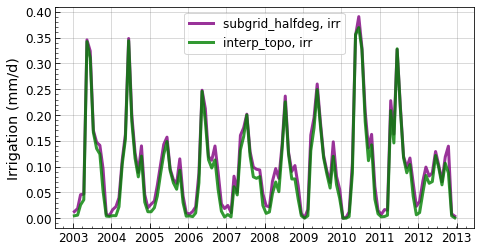
\includegraphics[width=\linewidth]{images/eval_halfdeg/time_series/irrigation_time_series.png}
    \end{subfigure}    
    \begin{subfigure}[b]{0.48\textwidth}
        \caption{}
        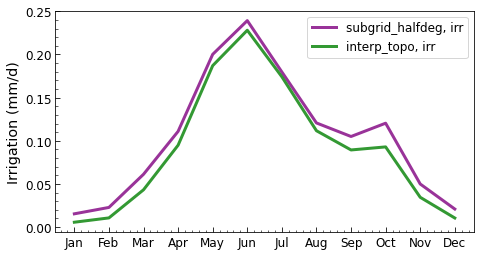
\includegraphics[width=\linewidth]{images/eval_halfdeg/time_series/irrigation_seasonal_cycle.png}
    \end{subfigure}

    \caption{Simulated irrigation in \std and \native. Annual mean for both simulations (a,b) and difference (c). Average time series (d) and seasonal cycle (e) over the Iberian Peninsula.}
    \label{fig:irrigation_halfdeg_eval}
\end{figure}

Both simulations show a similar simulated irrigation (Fig. \ref{fig:irrigation_halfdeg_eval}a, b), but the differences on reservoir volumes affect the available water, and therefore irrigation. This is particlarly visible in the Ebro valley where some grid cells are highly irrigated in one simulation and not in the other. This is due to the aforementionned differences in the routing graph, which affect the path of the Ebro river (Fig. \ref{fig:irrigation_halfdeg_eval}c), the main source for irrigation withdrawals in the region.
On average over the domain (Fig. \ref{fig:irrigation_halfdeg_eval}d, e) \std exhibits slightly higher volumes of irrigation than \native, which is consistent with the higher volumes in the river reservoir. As previously explained, the differences seen in the reservoirs on coastal grid cells seem to have little impacts on the irrigated volumes, since these regions are seldom intensely irrigated. %todo:ref to irrigmap figure ? In methods ?
%todo: comment more on depletion, irrigation limited by available water, and second peak in autumn which is enabled by new rain

%figure : river discharge seasonal cycle for 4 stations (large rivers but not Guadalquivir...), 2 routing versions, irr and no_irr for each
\begin{figure}[htbp]
    \centering
    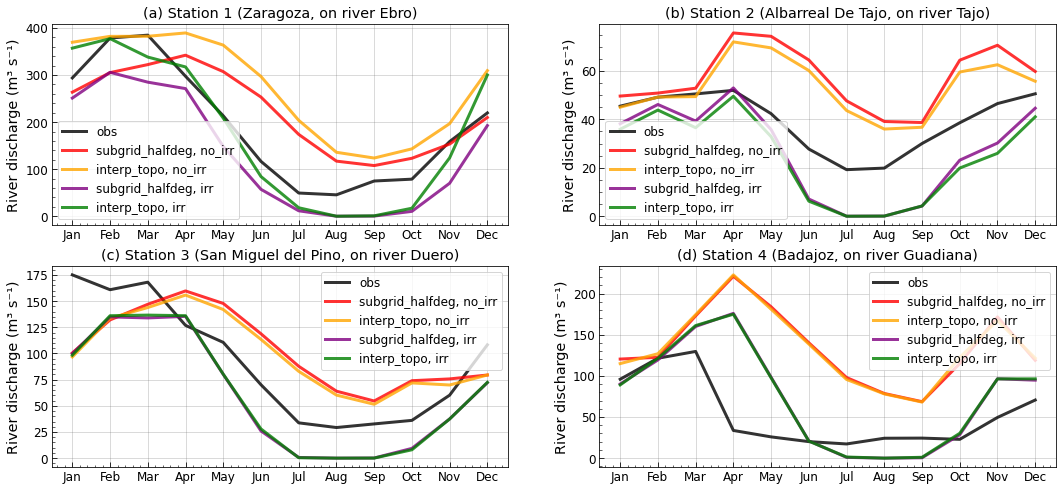
\includegraphics[width=\linewidth]{images/eval_halfdeg/river_discharge/halfdeg_4stations_SC.png}
    \caption{River discharge mean seasonal cycle (2003-2012) for 4 large stations of the Peninsula.}
    \label{fig:halfdeg_stations_SC}
\end{figure}

The seasonal cycle of river discharge reflects the general agreement of the two routing versions, without irrigation, the red and yellow lines follow each other closely, and with irrigation, the purple and green are also very similar. Some differences persist, due to the differences in the routing graph already described, mostly for the Ebro river since the station is downstream of several discrepancies visible on Fig. \ref{fig:routing_reservoirs_halfdeg}l.

\subsection{Conclusions}

This comparison of the \native routing version with \std showed that this new version is generally reproducing the modelling principles correctly, but several differences were identified between the two versions. All three reservoirs are handled differently in \native on coastal grid cells, which affects the average volumes stored over the Iberian Peninsula, but does not have a significant impact on irrigation or river dicharge. However, differences in the path followed by water as it flows from one grid cell to another in the river reservoirs are also clearly identified in large rivers of the Peninsula. This leads to local changes in the simulated river dicharge, and slightly less water stored in the river reservoir by \native since it simulated shorter paths in several occurrences. These discrepancies also have an impact on irrigation since it is strongly reliant on the volumes of water available in the river reservoir, but this impact remains limited on average over the domain.

\section{Calibration over the Iberian Peninsula}
\label{section:calib}

Once the general consistency of the \native routing had been assessed, it became possible to evaluate the specific setup that would be used for the coupled simulation, using the MERIT DEM at 2km resolution and accounting for irrigation. To use irrigation, the routing time step must be the same as the time step of ORCHIDEE, which is 15mn (900s) in coupled simulations. 

This calibration was initially focused on the three time constants of the routing reservoirs: TCST\_SLOW, TCST\_FAST, TCST\_STREAM. Although these parameters could theoretically be independent of the spatial and temporal time steps and of the DEM used as input, they can strongly influence the results. In particular, the ORCHIDEE routing scheme had never been used with a high-resolution topography like the MERIT DEM at 2-km resolution, since the \std routing ran only with the 0.5° resolution DEM used in the previous section, and often with a 24-hours routing time step. Multiple tests were therefore carried to identify an appopriate set of time constants for the reservoirs.
Moreover, the sensitivity of river discharge to the activation of irrigation was identified as very important, with large differences in the responses depending on the intensity of irrigation demand. As a consequence, the parameter $\beta$, which defines the soil moisture target in the irrigation scheme, was also included in this calibration and modified compared to the default version of the model.

% For these offline calibration simulations, given the better availability of flow observations and meteorological forcings before 2014, I did not work exactly on the period 2010-2022 but rather on the previous decades.. 

% It is also the version that was used for the calibration of the irrigation scheme developped in \citet{arboleda-obando_validation_2024} and since the scheme withdraws

\subsection{Simulation setup}

At the begining of the calibration, three reference sets of TCST parameters (presented in Table \ref{table:tcst_refs}) were considered:
\begin{itemize}
\item The values established during an initial calibration of the \native routing performed over the Danube basin, which focused only on river discharge observations \citep{kilic_evaluation_2023}.
\item The default values used by the \std routing on a global scale, which were used in the previous section with the 0.5° DEM. These values were identified empirically by a calibration study over the Senegal river basin and validated globally in \citet{ngo-duc_validation_2007} %todo:add ngoduc 2005
using river discharge and groundwater measurements from Gravity Recovery and Climate Experiment (GRACE) satellite data.
\item The values used for regional studies with the \textit{subgrid\_HTU} routing \citep{rinchiuso_improving_2022, huang_multi-objective_2024}.
\end{itemize}

\begin{table}[h]
\centering
\begin{tabular}{|l|c|c|c|}
\hline
\textbf{} & \textbf{TCST\_SLOW} & \textbf{TCST\_FAST} & \textbf{TCST\_STREAM} \\ \hline
Initial \native calibration & 1.2 & 0.9 & 0.03 \\ \hline
\std default values & 25 & 3 & 0.24 \\ \hline
\textit{Subgrid\_HTU} calibration & 600 & 80 & 6.3 \\ \hline
\end{tabular}
\caption{Reference parameter sets considered to calibrate the \native routing ($day \cdot km^{-1}$).}
\label{table:tcst_refs}
\end{table}

In these three sets of values, there is approximately an order of magnitude between the three time constants, and very significant differences (one or two orders of magnitude) between each set. 
This can be explained by the different DEMs used, the way HTUs are defined, and the calibration choices that led to these sets of values.%todo:compléter ? 

Three initial experiments were defined, based on these ratios:\\$TCST\_SLOW \approx 10 \times TCST\_FAST \approx 100 \times TCST\_STREAM$.
Table \ref{table:tcst_exp} presents these three sets of values based on the orders of magnitude of each of the reference value sets (TCST1, TCST2, TCST3), as well as the one selected after the calibration (TCST4), whose development steps are detailed hereafter.

\begin{table}[h]
\centering
\begin{tabular}{|l|c|c|c|}
\hline
\textbf{} & \textbf{TCST\_SLOW} & \textbf{TCST\_FAST} & \textbf{TCST\_STREAM} \\ \hline
TCST1 & 3 & 0.3 & 0.03 \\ \hline
TCST2 & 30 & 3 & 0.3 \\ \hline
TCST3 & 300 & 30 & 3 \\ \hline
TCST4 & 700 & 100 & 0.1 \\ \hline
\end{tabular}
\caption{Value sets of the simulations for the calibration of the \native routing ($day \cdot km^{-1}$).}
\label{table:tcst_exp}
\end{table}

Four simulations were therefore carried out with these four sets of TCST values, over the period 2000-2012, without activating irrigation.
The first three years are considered as a spin-up to allow the vegetation, soil moisture, and routing reservoir volumes to reach equilibrium, and the results presented therefore cover 10 years of simulation (2003-2012). %todo:remove if this part is already mentionned in the chapter methods

\subsection{Reservoir volumes and time constants}

%figure : 3 time series (3 reservoirs) on average over the IP for 4 tcsts and std as reference
%todo:subcaptions
\begin{figure}[htbp]
    \centering
    \begin{subfigure}[b]{0.32\textwidth}
        \caption{}
        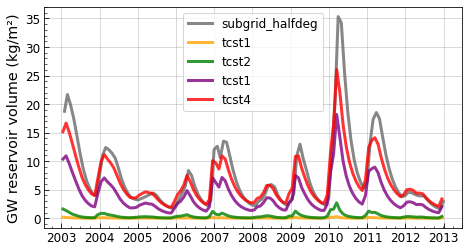
\includegraphics[width=\linewidth]{images/eval_halfdeg/time_series/slowr_time_series_tcsts.png}
    \end{subfigure}
    \begin{subfigure}[b]{0.32\textwidth}
        \caption{}
        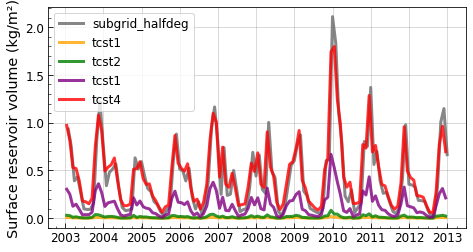
\includegraphics[width=\linewidth]{images/eval_halfdeg/time_series/fastr_time_series_tcsts.png}
    \end{subfigure}
    \begin{subfigure}[b]{0.32\textwidth}
        \caption{}
        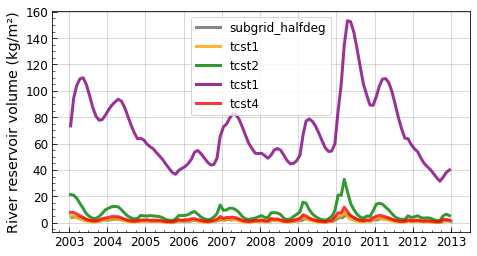
\includegraphics[width=\linewidth]{images/eval_halfdeg/time_series/streamr_time_series_tcsts.png}
    \end{subfigure} \\

    \begin{subfigure}[b]{0.32\textwidth}
        \caption{}
        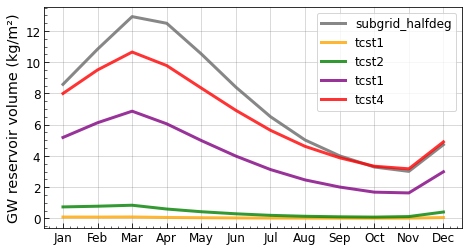
\includegraphics[width=\linewidth]{images/eval_halfdeg/time_series/slowr_seasonal_cycle_tcsts.png}
    \end{subfigure}
    \begin{subfigure}[b]{0.32\textwidth}
        \caption{}
        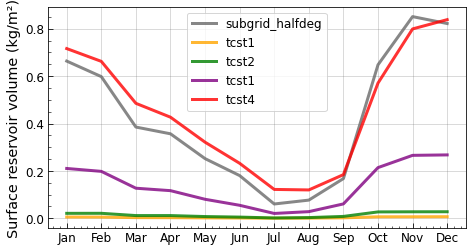
\includegraphics[width=\linewidth]{images/eval_halfdeg/time_series/fastr_seasonal_cycle_tcsts.png}
    \end{subfigure}
    \begin{subfigure}[b]{0.32\textwidth}
        \caption{}
        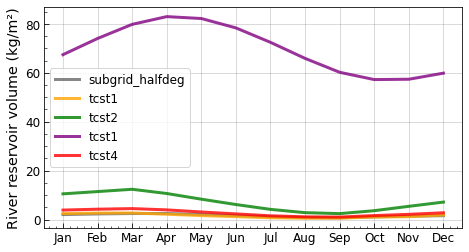
\includegraphics[width=\linewidth]{images/eval_halfdeg/time_series/streamr_seasonal_cycle_tcsts.png}
    \end{subfigure}
    \caption{Time series and seasonal cycles of reservoir volumes on average over the Iberian Peninsula domain.}
    \label{fig:reservoir_time_series_tcsts}
\end{figure}

%figure : river discharge seasonal cycle for 4 stations (large rivers but not Guadalquivir...), 2 routing versions, irr and no_irr for each
\begin{figure}[htbp]
    \centering
    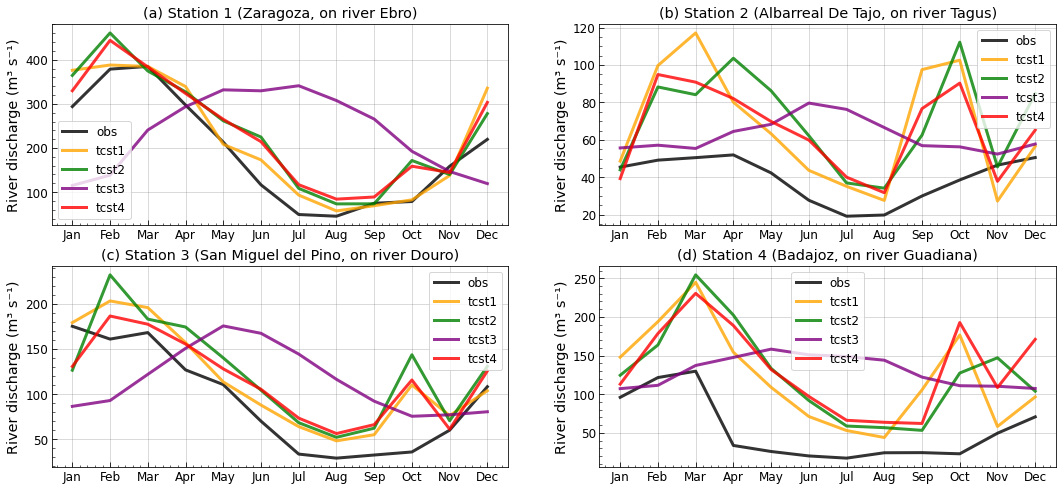
\includegraphics[width=\linewidth]{images/eval_halfdeg/river_discharge/merit_tcst_4stations_SC.png}
    \caption{River discharge mean seasonal cycle (2003-2012) for 4 large stations of the Peninsula.}
    \label{fig:merit_tcsts_stations_SC}
\end{figure}

\subsection{Impact of irrigation on river discharge}

blabla
blabla

blabla


\begin{figure}[htbp]
    \centering
    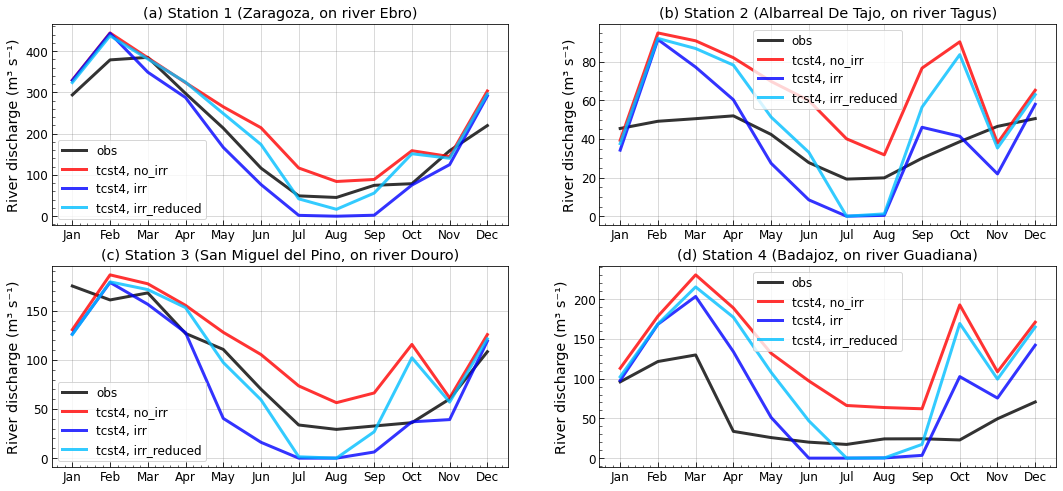
\includegraphics[width=\linewidth]{images/eval_halfdeg/river_discharge/merit_irr_4stations_SC.png}
    \caption{River discharge mean seasonal cycle (2003-2012) for 4 large stations of the Peninsula.}
    \label{fig:merit_irr_stations_SC}
\end{figure}

\subsubsection{Sensitivity to atmospheric forcing}


\begin{figure}[htbp]
    \centering
    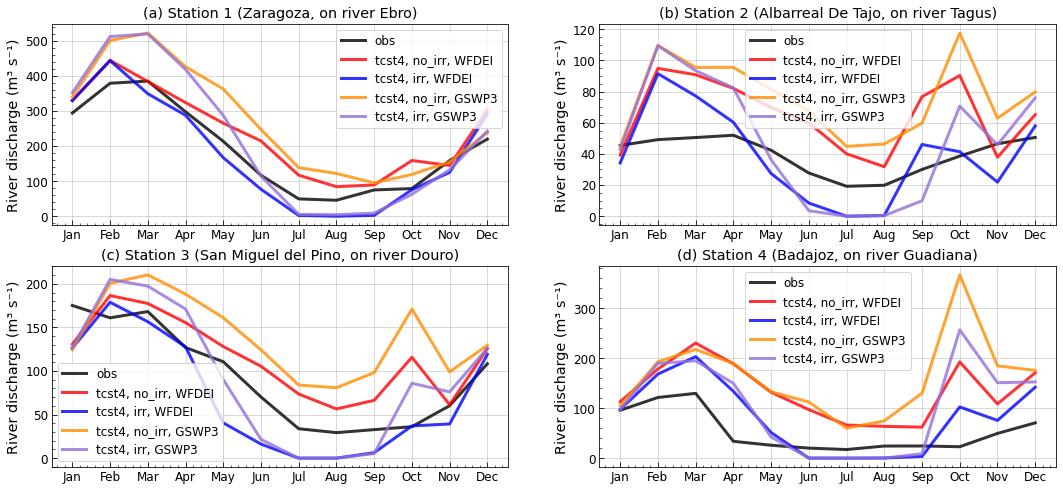
\includegraphics[width=\linewidth]{images/eval_halfdeg/river_discharge/merit_forcing_4stations_SC.png}
    \caption{River discharge mean seasonal cycle (2003-2012) for 4 large stations of the Peninsula.}
    \label{fig:merit_forcing_stations_SC}
\end{figure}

\section{Chapter conclusions}

This chapter presents the evaluation and calibration of the new version of the routing scheme using ORCHIDEE offline simulations  over the Iberian Peninsula, which was necessary to prepare for coupled simulations.

This calibration and evaluation work first showed that the new routing code behaves similarly to the pre-existing version if given the same input map and parameters.%todo : some differences identified ?

The new routing was then used with a high-resolution DEM over the Iberian Peninsula, and several options were tested for the reservoir time constants. 
Comparison of reservoir volumes with the previous version of the routing (\std), which served as a first reference, allowed the identification of values for TCST\_SLOW and TCST\_FAST to simulate similar water volumes on average over the Peninsula. This was essential because of the dependance of the irrigation scheme on the available water in the routing reservoirs.
Using discharge observations, the value of TCST\_STREAM was then adjusted to correctly represent the seasonal cycle of the major rivers of the Iberian Peninsula.

Sensitivity experiments highlighted the very large response of river discharge to the activation of irrigation (except in winter). 
This is not shown here, %tocheck and/or todo
but it is worth noting that irrigation stood out significantly compared to other sensitivity analyses conducted (on meteorological forcing, on the use of bare soil evaporation resistance). 
The magnitude of this sensitivity also contributed to the decision not to further calibrate the TCST values, whose impact on fidelity to observations remains limited compared to that of irrigation.
As a consequence, the $\beta$ parameter of the irrigation scheme was also included in the calibration, and 0.6 was identified as a more suitable value than the default 0.9. This choice allows avoiding excessively low discharge in summer for the four rivers considered, and is considered more consistent with a representation of irrigation practices in the region.

Therefore, the set of parameters from the simulations \textit{tcst4\_no\_irr} and \textit{tcst4\_irr\_reduced} were used to study the impact of irrigation in the coupled simulations presented in CHapter \ref{chap:monthly}.
%over